\section{绪论}
\subsection{背景研究}
2016年7月,中共中央、国务院办公厅印发了《国家信息化发展战略纲要》,规范和指导了未来10年中央对国家信息化的指导思想和战略方针。信息技术的基础水平和相关产业的发展程度,与国家信息化进程密切相关。《国信纲要》提倡,要加强信息技术领域前沿和基础研究,同时应用相应技术,打造协同发展的产业生态。2020年5月两会期间,多位人大代表和政协委员提出了,关于区块链技术在产业中的应用、促进产业发展升级和数字货币监督监管问题,三大方面的想法与提议。由此可知,区块链已然成为了当下乃至今后十年内,我国科技、信息领域发展的“顶层设计”。在这样的发展潮流下,区块链的落地应用和技术推广如雨后春笋:国家邮政局鼓励以区块链为主要应用核心的新一代技术升级;银保监会为提高数据安全性,在交易环节应用区块链技术;教育部也在《全国大中小学教材建设规划(2019-2022年)》的记者问答中表示,下一步将围绕区块链等新技术领域重点建设,集中力量编写、打造新经典教材。

2020年初的疫情导致近乎所有学生都参与到了线上教学,由此影响,在线课堂、在线考试受到了极大的推广。腾讯会议、钉钉、腾讯课堂等线上视频会议的产品快速迭代之中逐渐成熟。与之相应,也诞生了许多在线考试的相关解决方案,例如超星学习通、中国大学慕课、智慧树。线上考试的方式与传统的线下纸质化考试相比,有如下的优劣之处:

\begin{itemize}
    \item 能够代替教师的部分工作,一定程度上地方便学校、教育机构对考试的安排管理,提高了工作效率;
    \item 有效地缩短考试前期安排的组织周期,减轻了相关通知传递过程中的人力损耗;
    \item 线上交卷、评卷缩短了学生得到考试反馈结果的时间周期;
    \item 在相关硬件设施条件满足的前提下,进一步地保证了考试过程中的公平公正;
    \item 存在线上系统都无法避免的网络攻击风险;
    \item 数据集中化存储管理,有潜在的被篡改等安全问题;
\end{itemize}

如上的在线考试解决方案通常使用了移动端 C/S 结构,桌面端 B/S 结构。如此的客户端-服务端解构模式,实现了在不同的用户前端实现下,用户数据的共通。在这样的项目架构模型中,数据的安全性、可靠性、可信度便显得尤为关键。结合这两个方面,提出本项目「基于区块链技术的线上考试系统」。线上考试系统的方式合理利用了当今时代互联网的便捷性与普及程度。采用国家大力支持推广的区块链技术,可以有效地保证数据存储管理的安全性。

区块链技术最早由中本聪于《比特币:一种点对点的电子现金系统》\textsuperscript{\cite{ref0}}一文中提出,是一种类似于分布式的账本的数据存储与管理技术。在共识机制、工作量证明(PoW)等方式保障下,区块链技术具有:不可篡改、可追溯源、去中心化等特性与优点。这些特点正好与线上考试系统的数据安全方面的问题十分契合:防篡改、可溯源保证了考试数据的安全;去中心化的特性发挥了数据分布式存储的优势,降低了集中化数据存储方式存在的安全风险,减轻了系统服务器压力,加强了数据可用性、系统可用性。将区块链技术应用至系统中,会是诸如线上考试系统此类的数据安全敏感系统今后的更新趋势,也呼应了国家对于区块链技术重视与号召。


\subsection{需求分析}
\subsubsection{目标用户群体}
\begin{itemize}
    \item 学校、教育机构:有固定时间周期性的测试或考试需要,使用线上考试系统可以覆盖一些简单的定期多次小测验;
    \item 学生:无纸化的线上考试系统使得考试结果反馈更加快速;
\end{itemize}

\subsubsection{用户主要目的}
需要一款线上考试系统的解决方案,能方便快捷的满足学校、教育机构平时周期性的测试的需要。教师能够简单的操作就能配置题目、题库、发布试卷,通过预先设定的参考答案,能够自动评卷登分,将考试结果与相关题目解析快速反馈给参与考试的学生。

\subsubsection{功能性需求}
\begin{figure}[htb!]
    \centering
    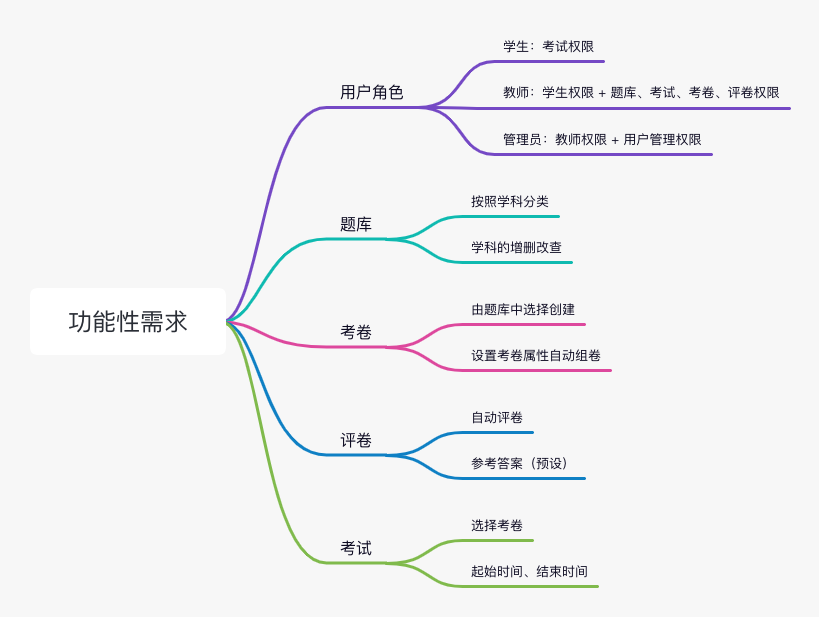
\includegraphics[width=0.8\linewidth]{_images/功能性需求.png}
    \caption{功能性需求}
    \label{功能性需求}
\end{figure}
\paragraph{用户角色分类} 系统的参与者主要分为三类:学生、教师、管理员,学生与教师对应实际业务场景中的角色,管理员是因系统的操作与非业务的操作而存在。
\paragraph{题库功能} 题目作为考卷的基本单位,考卷就是多个题目的组成。项目需要题目的基本管理功能。题目按题型又将分为:单选题、多选题、判断题、填空题等。题目按照学科分类,因此又需要题库功能对不同的学科题目进行管理。
\paragraph{考卷功能} 考卷是考试进行的必要组成部分,考卷需要由教师手动从题库中选择,或是通过设定一定的规则从设定好的题库中抽取自动组卷。考卷也需要基本的增删改查功能。
\paragraph{考试功能} 考试通过选择已创建的考卷而开启,学生可以进入已创建的考试进行线上考试。考试也需要设置起始时间和结束时间属性。
\paragraph{评卷功能} 题目设置的时候提供对应的正确答案选项,使得在作答结束后能够通过正确答案与学生的作答情况自动评卷计分,并提供预先设置的参考题解给学生。
\paragraph{用户管理} 管理员才被允许对系统中的用户进行新增、删除、修改信息、查看。用户也可以对自己的基本信息做修改,例如修改密码、头像、昵称。
\paragraph{权限分类} 根据以上的用户角色分类和功能模块,需要将具体的功能模块访问限制与用户角色对应。学生只允许参与考试和查看自己考试的情况;老师具有学生的所有权限用于考卷的试测,此外需要考卷功能模块、题库功能模块、评卷功能模块的权限;管理员具有所有的功能模块权限,即老师的权限加上用户管理功能模块的权限。

\subsubsection{非功能性需求}
\begin{itemize}
    \item 界面美观,布局简洁大方;
    \item 用户交互操作友好。用户意外的错误操作,或是发生运行时错误,应有合理的信息提示;
    \item 系统使用需要有清晰、完善的文档说明,项目代码注释完善、易读;
    \item 项目需要具有足够的测试性,以保证系统性能可用于实际环境;
    \item 项目结构设计良好、易于维护,并留存有一定后期功能拓展的空间;
    \item 用户操作具有完备的鉴权流程,防止非法操作;
    \item 前端布局弹性,根据不同的分辨率响应式渲染展示;
\end{itemize}


\subsection{进度安排}
\paragraph{2021/1/8 - 2021/2/28} 确定选题,查阅文献,外文翻译和撰写开题报告。这期间主要通过导师提供的相关材料,以及自己查阅相关的文献,熟悉项目题目的研究背景、应用领域、技术生态。在完成了文献查阅和外文文献翻译后,根据自己的这阶段对项目选题的方方面面的理解,撰写开题报告;
\paragraph{2021/3/1 - 2021/3/20} 完成系统核心功能设计,主要包括数据库表设计,对项目中实体的抽象;使用 Vue 及其相关技术栈实现最小 Demo,主要目的是通过实际开发实践巩固所学的前端技术部分的理论知识;熟悉 SpringBoot、Fisco Bcos 等后端部分的技术文档,对业务对象、功能模块的设计实现有一定思考和初步设想,能做到胸有成竹;
\paragraph{2021/3/21 - 2021/4/20} 参考网上成熟的系统界面原型设计,对前端部分的布局和组件抽象有大概的构想;编写项目的核心功能模块的代码,包括前端页面展示部分和后端数据处理部分;
\paragraph{2021/4/21 - 2021/5/11} 尝试与实践区块链的结点部署,并修改项目后端核心实体对象的数据处理,增加区块链接入层,实现安全敏感的重要数据上链;
\paragraph{2021/5/12 - 2021/5/18} 熟悉相关的测试技术,对项目进行单元测试、压力测试等各方面的测试,并记录数据;
\paragraph{2021/5/19 - 2021/5/31} 撰写及修改毕业论文;
\paragraph{2021/6/1 - 2021/6/5} 准备答辩。

\subsection{论文结构安排}
\paragraph{第一章}绪论介绍了在当下的社会政策与技术潮流中,项目的研究和应用意义。以及分析了项目面向的用户群体,用户需求。

\paragraph{第二章}简要介绍了项目所使用的相关技术栈,简要概述了技术选型的思考过程:选用的技术的稳定程度与社区生态;与相似技术及其技术栈对比之中的优劣;与项目开发的适用性。

\paragraph{第三章}介绍了系统的整体设计模型、分层的构思过程,项目系统具体的分工模块,模块间的相互协作。

\paragraph{第四章}重点着眼于项目系统的几个核心模块的代码实现思路,和模块的代码开发中所遇到的难点、个人的思考与解决方式。

\paragraph{第五章}展示了使用相关的测试技术对项目应用时各方面的测试结果与结论。

\paragraph{第六章}总述个人对于项目仍存在的不足之处,和潜在的改进空间。